% Hi! We're member of IRIS-HEP and the Scikit-HEP community project, where we are building
% a Pythonic data analysis ecosystem for HEP community.
% IRIS-HEP does lots of things from data delivery, to cyberinfrastructure, and supporting the
% development of existing software tools, and has been a community center for fostering Scikit-HEP
% development.
% A shared goal is that we want to empower analysts at the LHC and beyond with modern data science stacks
% and build powerful libraries that allow for analysts to build expressive analysis workflows.
% \begin{frame}{Hello from IRIS-HEP and Scikit-HEP!}
%   \begin{columns}
%     \column{0.6\textwidth}
%     \Large
%     % \begin{itemize}
%     \begin{itemize}\setlength{\itemsep}{0.5 cm}
%       \item We're members of the \href{https://iris-hep.org/}{Institute for Research and Innovation in Software for High Energy Physics (IRIS-HEP)} and the \href{https://scikit-hep.org/}{Scikit-HEP} community project developing a Pythonic data analysis ecosystem for HEP
%       \item Goals: Empower analysts with modern data science stacks and provide powerful libraries for building expressive workflows
%     \end{itemize}
% %
%     \column{0.4\textwidth}
%     \begin{figure}
%         \begin{center}
%             \href{https://iris-hep.org/}{
\includegraphics[width=0.9\linewidth]{iris-hep-logo-long.pdf}}
%             \href{https://scikit-hep.org/}{
\includegraphics[width=0.8\linewidth]{scikit-hep-logo.pdf}}
%         \end{center}
%     \end{figure}
%   \end{columns}
% \end{frame}

% \begin{frame}{Built with intentionality and interoperability}
%   \begin{columns}
%     \column{0.45\textwidth}
%     \begin{enumerate}\setlength{\itemsep}{0.5 cm}
%       \item[5] HEP-specific UI applications or packaged algorithms
%       \item[4] HEP-specific for common problems
%       \item[3] HEP-specific, foundational
%       \item[2] needed to create, but not really HEP-specific
%       \item[1] non-HEP software we depend on
%     \end{enumerate}
% %
%     \column{0.55\textwidth}
%     \begin{figure}
%         \begin{center}
%             \href{https://indico.cern.ch/event/1140031/}{\includegraphics[width=\linewidth]{shells-hep.pdf}}
%         \end{center}
%     \end{figure}
%   \end{columns}
% \end{frame}

\begin{frame}{Analysis Systems Team}
  \begin{columns}
    \column{0.4\textwidth}
    % \Large
    % \begin{itemize}
    \begin{itemize}\setlength{\itemsep}{0.1 cm}
      \item Wisconsin-Madison
      \begin{itemize}
        \item Kyle, Alex, Matthew
      \end{itemize}
      \item Washington
      \begin{itemize}
        \item Gordon, Mason, Tal
      \end{itemize}
      \item Princeton
      \begin{itemize}
        \item Jim, Henry, Ianna
      \end{itemize}
      \item University of Cincinnati
      \begin{itemize}
        \item Mike, Thomas
      \end{itemize}
      \item Illinois
      \begin{itemize}
        \item Mark, Ben
      \end{itemize}
      \item NYU
      \begin{itemize}
        \item Irina
      \end{itemize}
      \item University of Nebraska-Lincoln
      \begin{itemize}
        \item Oksana
      \end{itemize}
    \end{itemize}
%
    \column{0.6\textwidth}
    \begin{figure}
        \begin{center}
            \href{https://iris-hep.org/as.html}{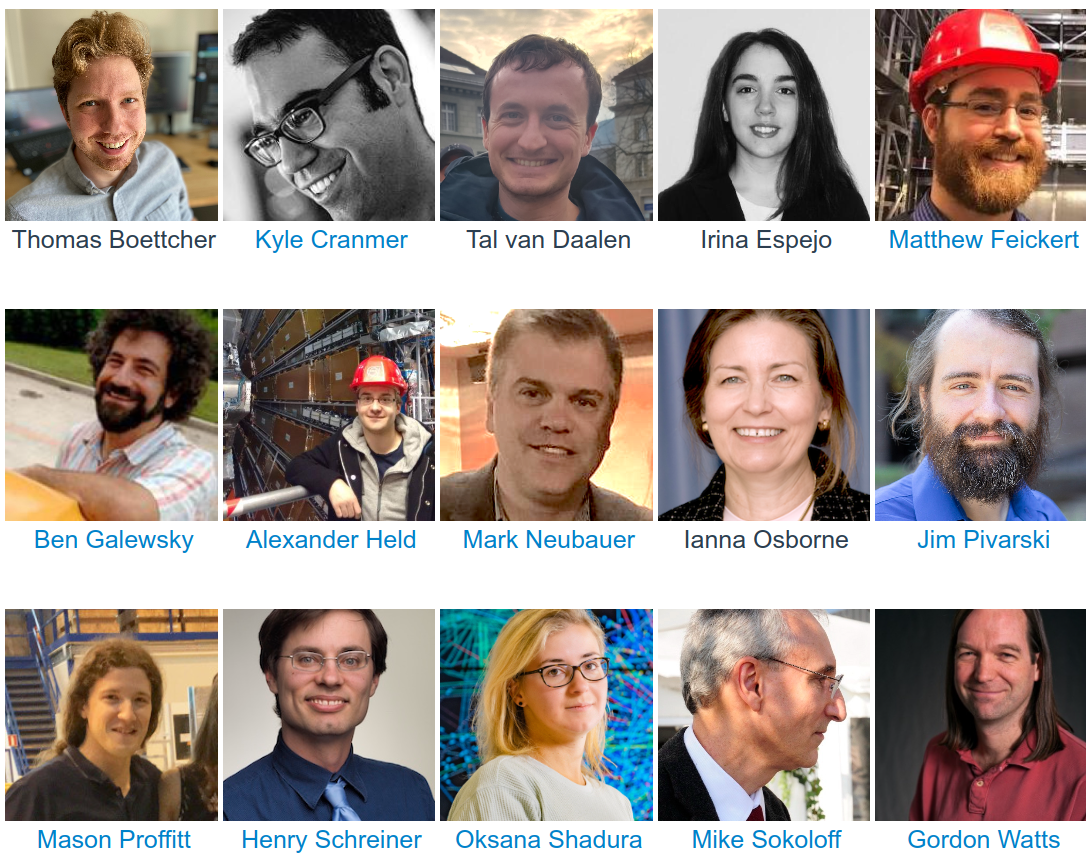
\includegraphics[width=\linewidth]{analysis-systems-team.png}}
        \end{center}
    \end{figure}
  \end{columns}
\end{frame}

\begin{frame}{Analysis Systems Projects}
  \begin{columns}
    \column{0.4\textwidth}
    % \begin{itemize}
    \begin{itemize}\setlength{\itemsep}{0.25 cm}
      \item Analysis Systems are connected to analysis use cases
      \item Systems are composed of components
      \item Large number of these projects refer to these componetns
      \begin{itemize}
        \item Many projects include people beyond IRIS-HEP directly
      \end{itemize}
      \item Milestones and activities are mainly oriented towards integration, evaluation, with a global overview of the vertical
    \end{itemize}
%
    \column{0.6\textwidth}
    \begin{columns}
      \begin{column}{0.5\textwidth}
        \begin{figure}
          \begin{center}
            \href{https://iris-hep.org/as.html}{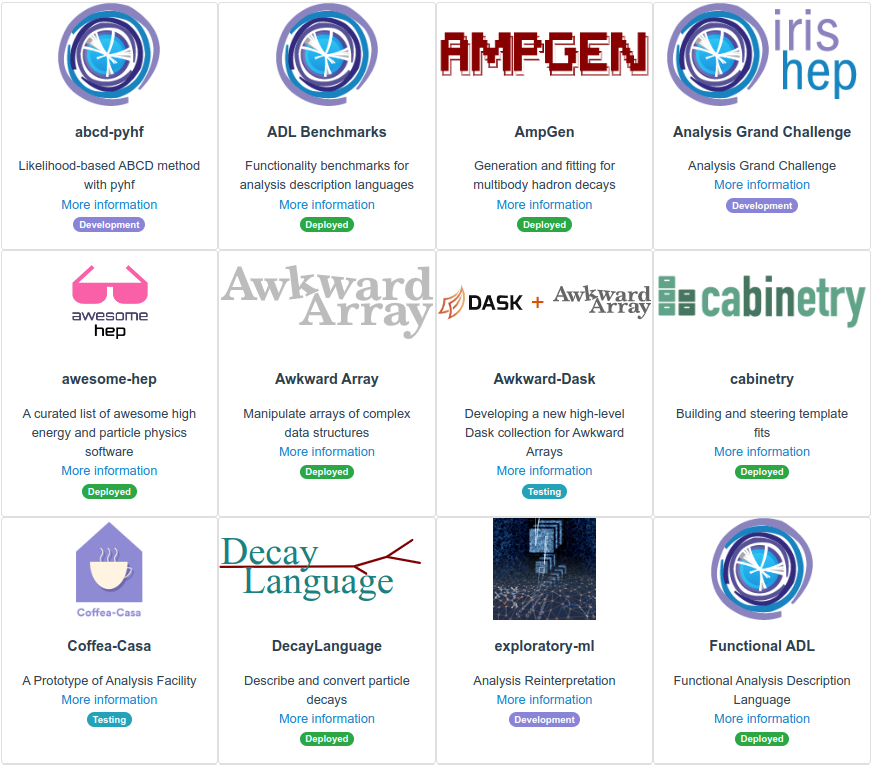
\includegraphics[width=\linewidth]{as_projects_1.png}}
          \end{center}
        \end{figure}
      \end{column}
      \begin{column}{0.5\textwidth}
        \begin{figure}
          \begin{center}
            \href{https://iris-hep.org/as.html}{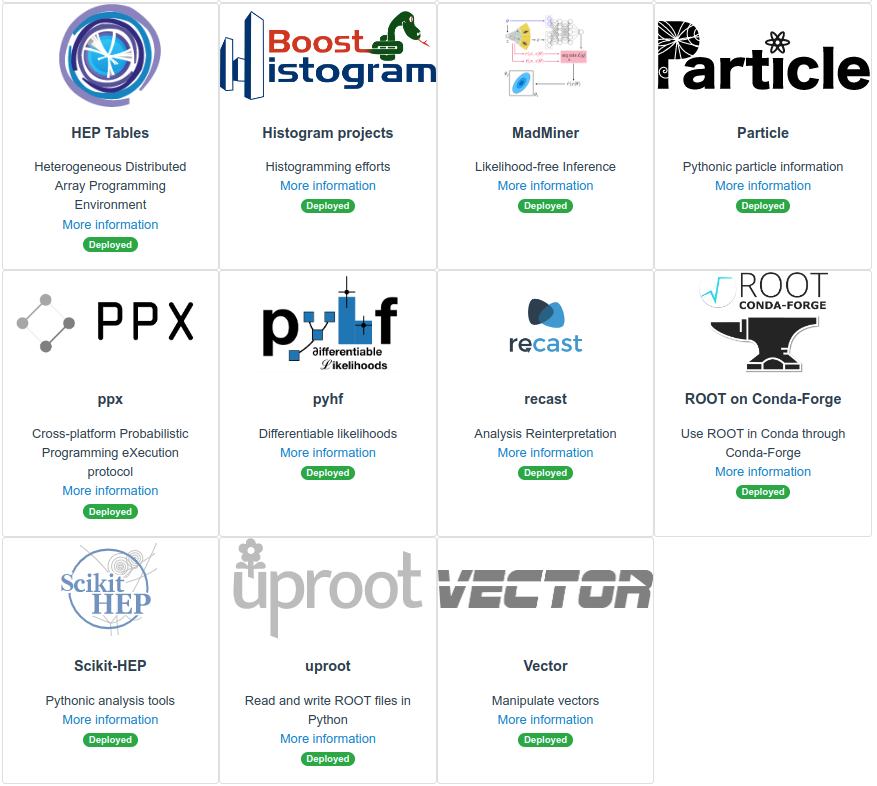
\includegraphics[width=\linewidth]{as_projects_2.png}}
          \end{center}
        \end{figure}
      \end{column}
    \end{columns}
    \begin{center}
      Analysis Systems Projects
    \end{center}
  \end{columns}
\end{frame}

\begin{frame}
  \frametitle{Analysis Systems Pipeline}

  \begin{figure}
    \begin{center}
      \href{https://iris-hep.org/as.html}{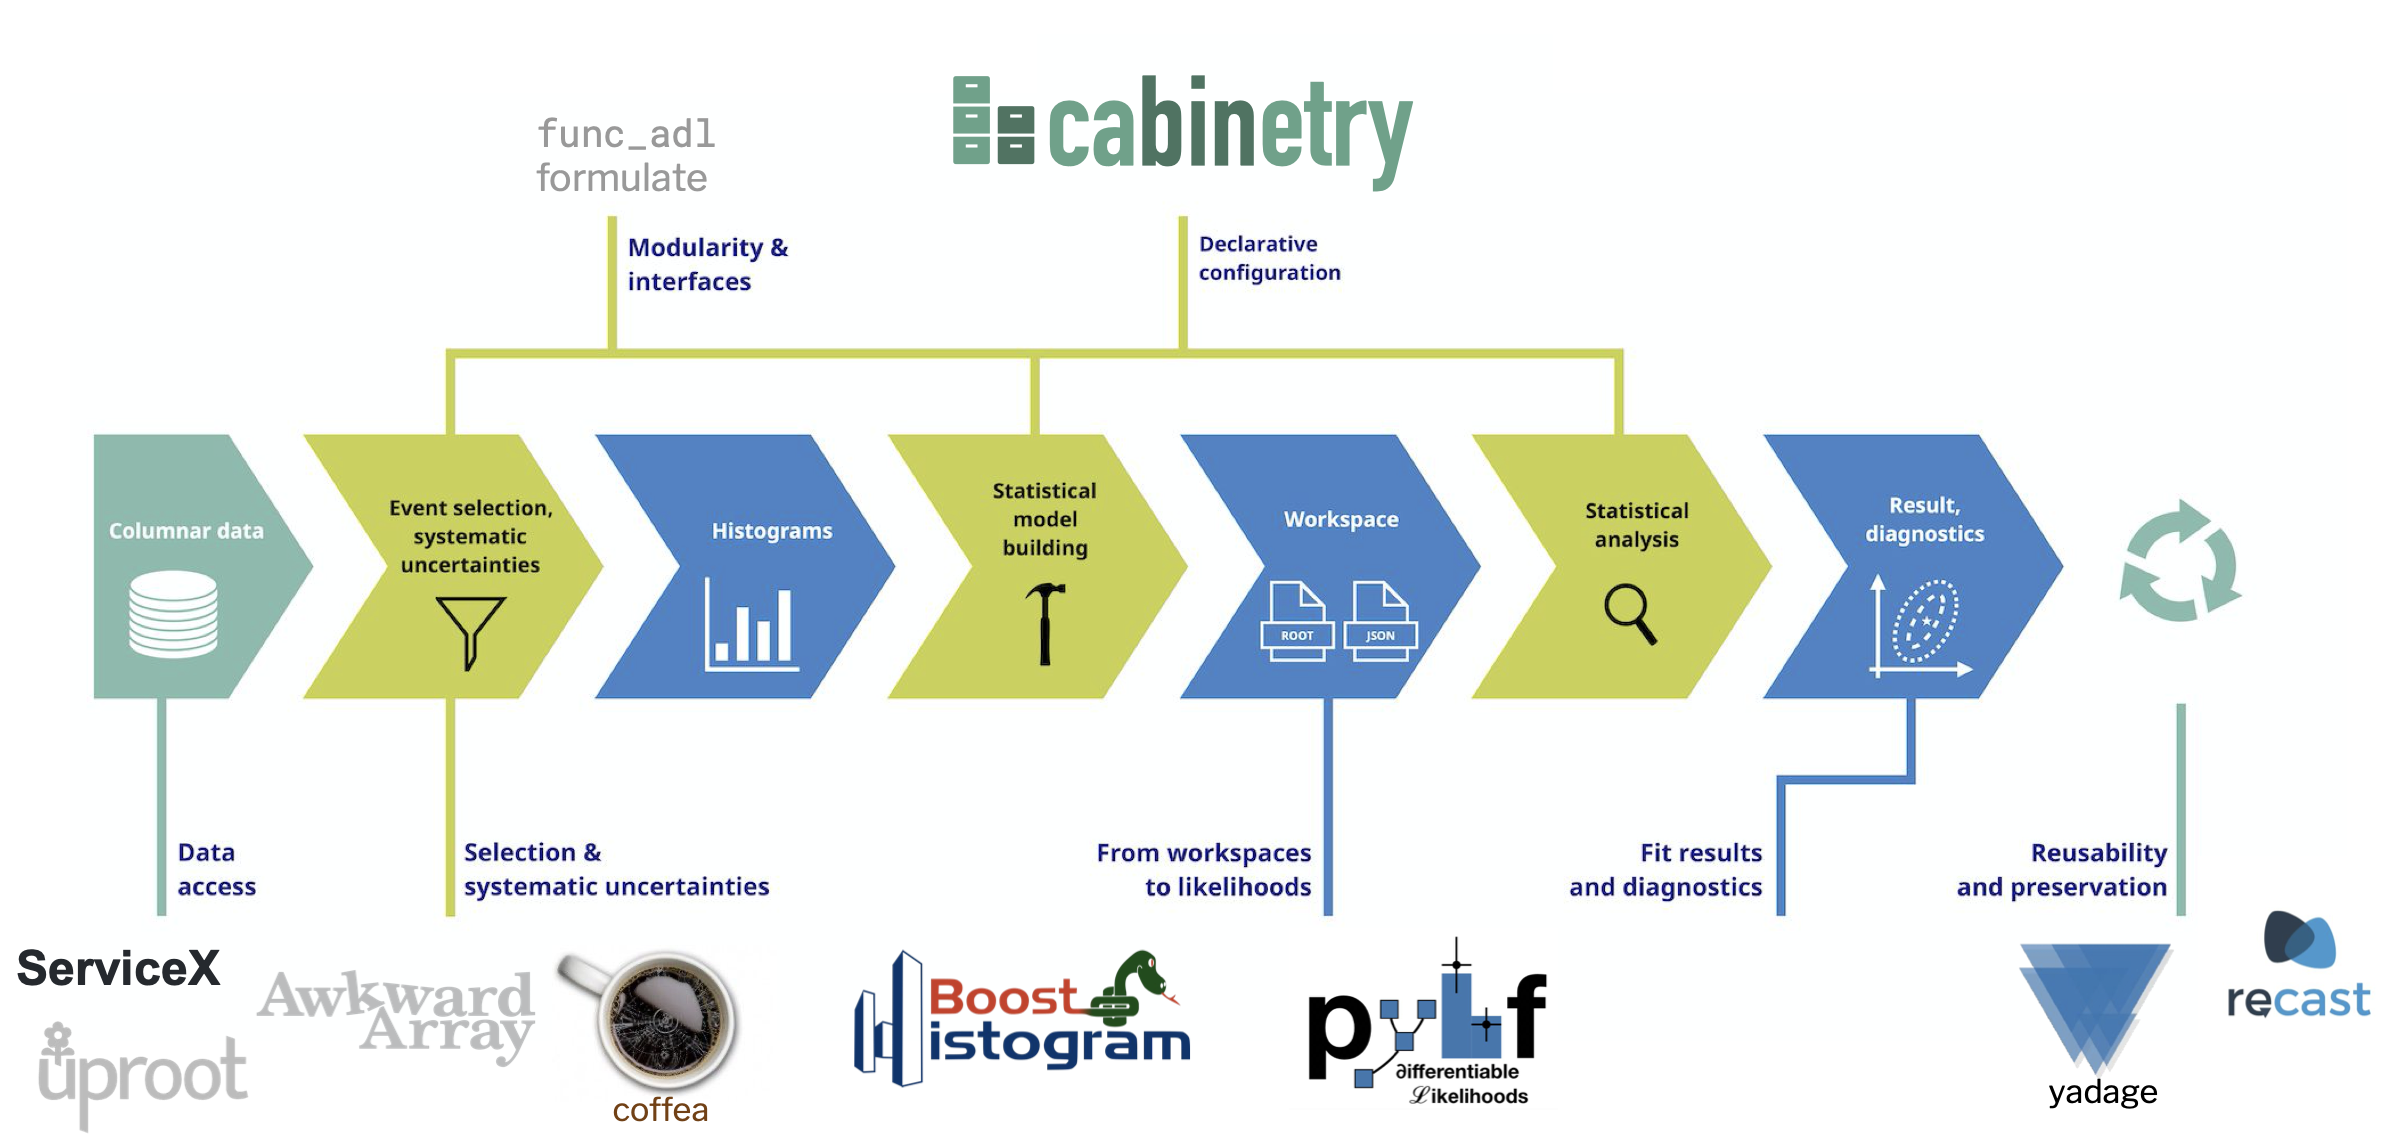
\includegraphics[width=0.75\linewidth]{cabinetry-vertical-slice.png}}
    \end{center}
  \end{figure}

  \begin{itemize}
    \item Together these project compose to form a coherent \textbf{analysis pipeline}
    \item Interface with \linkref{https://iris-hep.org/doma.html}{DOMA} (ServiceX, Coffea-Casa, and friends) and \linkref{https://iris-hep.org/ssl.html}{Scalable Systems Laboratory} (analysis facilities) areas, benefitting from \linkref{https://iris-hep.org/blueprint.html}{Blueprint Activity} process
    \item Underlying pipeline for the Anlaysis Grand Challenge (AGC)
    \begin{itemize}
      \item c.f. Alex and Oksana's \linkref{https://indico.cern.ch/event/985527/contributions/4635518/}{AGC update in Steering Board Meeting 12}
    \end{itemize}
  \end{itemize}

\end{frame}

\begin{frame}
  \frametitle{Analysis Systems Year 4 Themes}

  \begin{itemize}\setlength{\itemsep}{0.25 cm}
    \item \textbf{Year 3} focused on \textbf{Integration and Adoption}
    \begin{itemize}
      \item Getting tools to work coherently together and getting the community using them
    \end{itemize}
    \item Year 4
    \begin{itemize}
      \item \textbf{Project maturity / feature completness}
      \begin{itemize}
        \item (core) feature completness of \texttt{pyhf}, \texttt{cabinetry}
        \item Roadmaps for integration of Awkward to broader analysis communities (\linkref{https://iris-hep.org/projects/awkward-dask.html}{Awkward-Dask}) and differntiable analysis
      \end{itemize}
      \item \textbf{Community socialization / supporting analysis use}
      \begin{itemize}
        \item \texttt{pyhf} used in published analyses by ATLAS, Belle II, Belle, pheno community (35 use citations to date)
        \item Scikit-HEP tools finding traction outside of HEP (Awkward, boost-histogram)
        \item Scikit-HEP / IRIS-HEP tools and maintainers being invited to broader Scientific Python conferences and communities (SciPy Confrences, PyPA packaging summit)
        \item Adoption of pieces of ecosystem making it easier for the whole (uproot ubiquitous, ATLAS investigating Daks for analysis workflows, coffea adopts hist, LHCb publishes first analysis using only Scikit-HEP tools)
      \end{itemize}
    \end{itemize}
    % \item Lay out what the actual project goals are and where we're going here
    % \item Compare to the requirements that we've agreed to
  \end{itemize}

\end{frame}

\begin{frame}
  \frametitle{Analysis Systems Project Highlights: Awkward}

  \begin{columns}
    \column{0.45\textwidth}
    \begin{itemize}\setlength{\itemsep}{0.1 cm}
      \item Awkward is used outside of HEP, and very much appreciated
      \item \begin{figure}
        \begin{center}
            \href{https://iris-hep.org/projects/awkward-dask.html}{
\includegraphics[width=\linewidth]{awkward-dask.pdf}}
        \end{center}
    \end{figure}
        %
   Awkward Array CSSI (\linkref{https://www.nsf.gov/awardsearch/showAward?AWD_ID=2103945}{OAC-2103945}) has development of a new Dask container type representing Awkward Arrays
      \item
      \begin{figure}
        \begin{center}
            \href{https://github.com/jpivarski-talks/2022-07-11-scipy-loopy-tutorial}{
\includegraphics[width=\linewidth]{awkward-tutorial-placecard.png}}
            Part of Jim's SciPy 2022 Tutorial
        \end{center}
      \end{figure}
    \end{itemize}
%
    \column{0.55\textwidth}
    \begin{figure}
        \begin{center}
            \href{https://iris-hep.org/analysis-community-summary/\#stars}{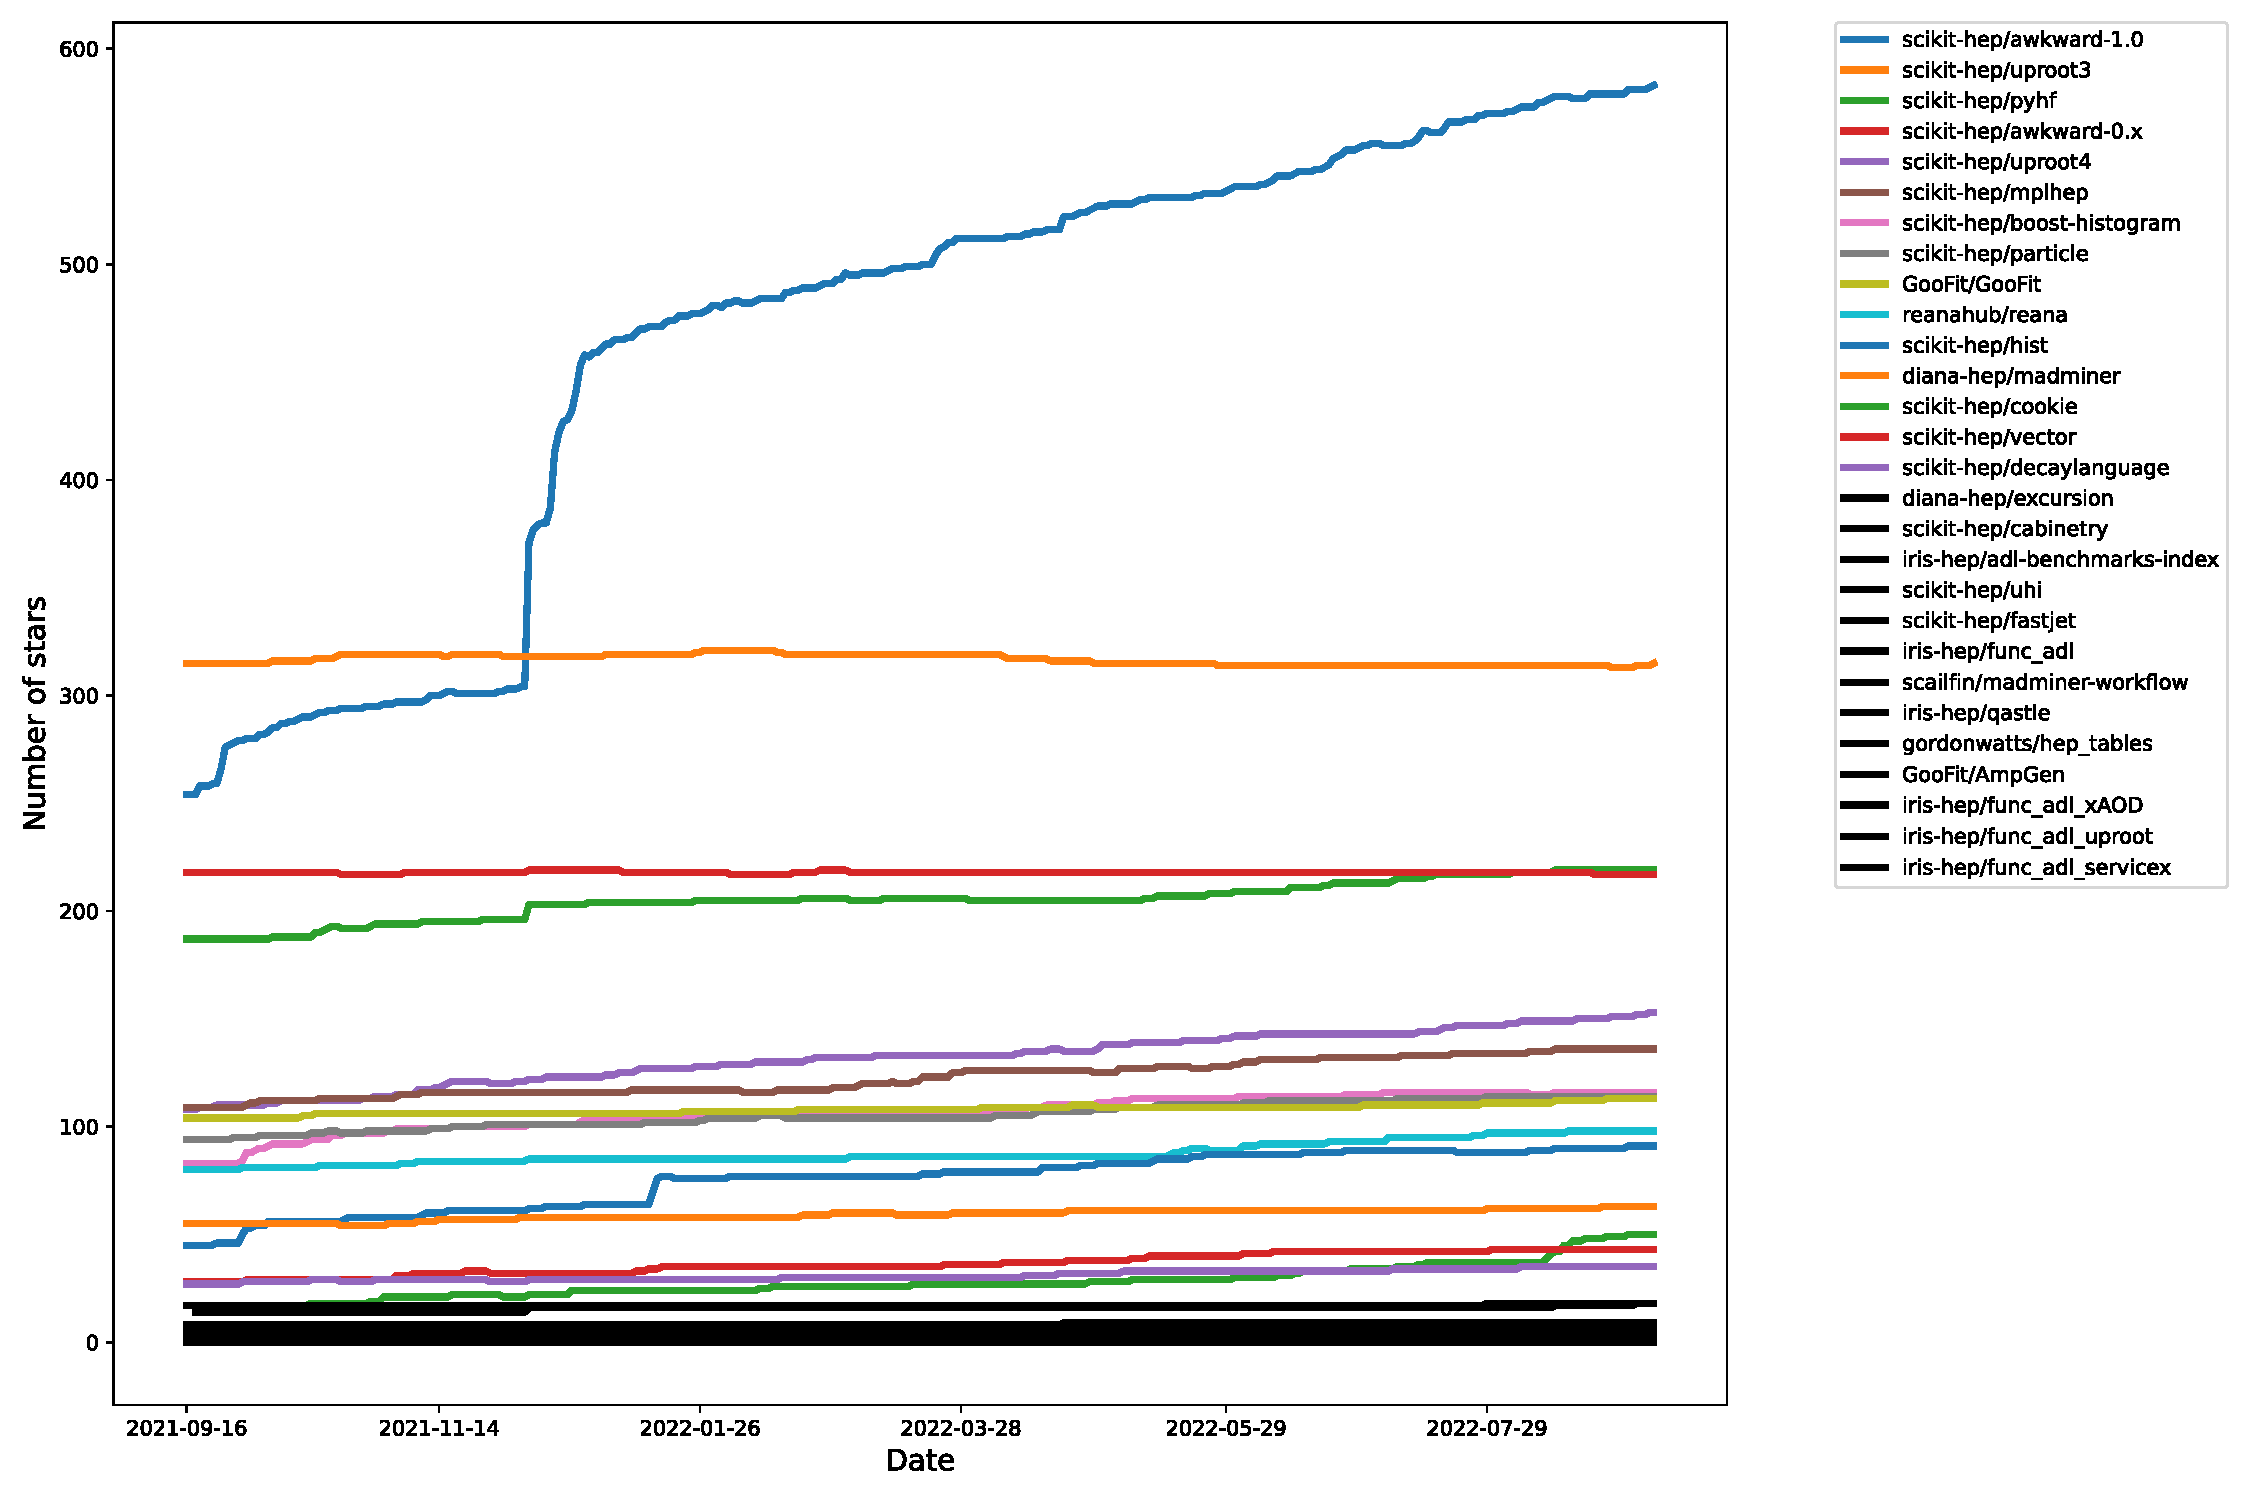
\includegraphics[width=\linewidth]{time_series_stars.pdf}}
            Cummulative GitHub stars of IRIS-HEP/Scikit-HEP projects vs. time. Awkward has the most by far.
        \end{center}
    \end{figure}
  \end{columns}

\end{frame}

\begin{frame}
  \frametitle{Analysis Systems Project Highlights: hist}

  \begin{columns}
    \column{0.45\textwidth}
    \begin{itemize}\setlength{\itemsep}{0.1 cm}
      \item hist is being adopted as the histogramming library of coffea
      \begin{figure}
        \begin{center}
          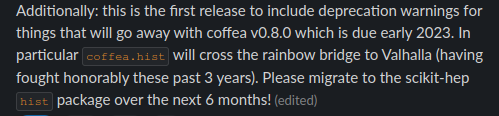
\includegraphics[width=\linewidth]{hist-adoption-in-coffea.png}
        \end{center}
      \end{figure}
    \end{itemize}
%
    \column{0.55\textwidth}
    \begin{figure}
        \begin{center}
            \href{https://github.com/jpivarski-talks/2022-07-11-scipy-loopy-tutorial}{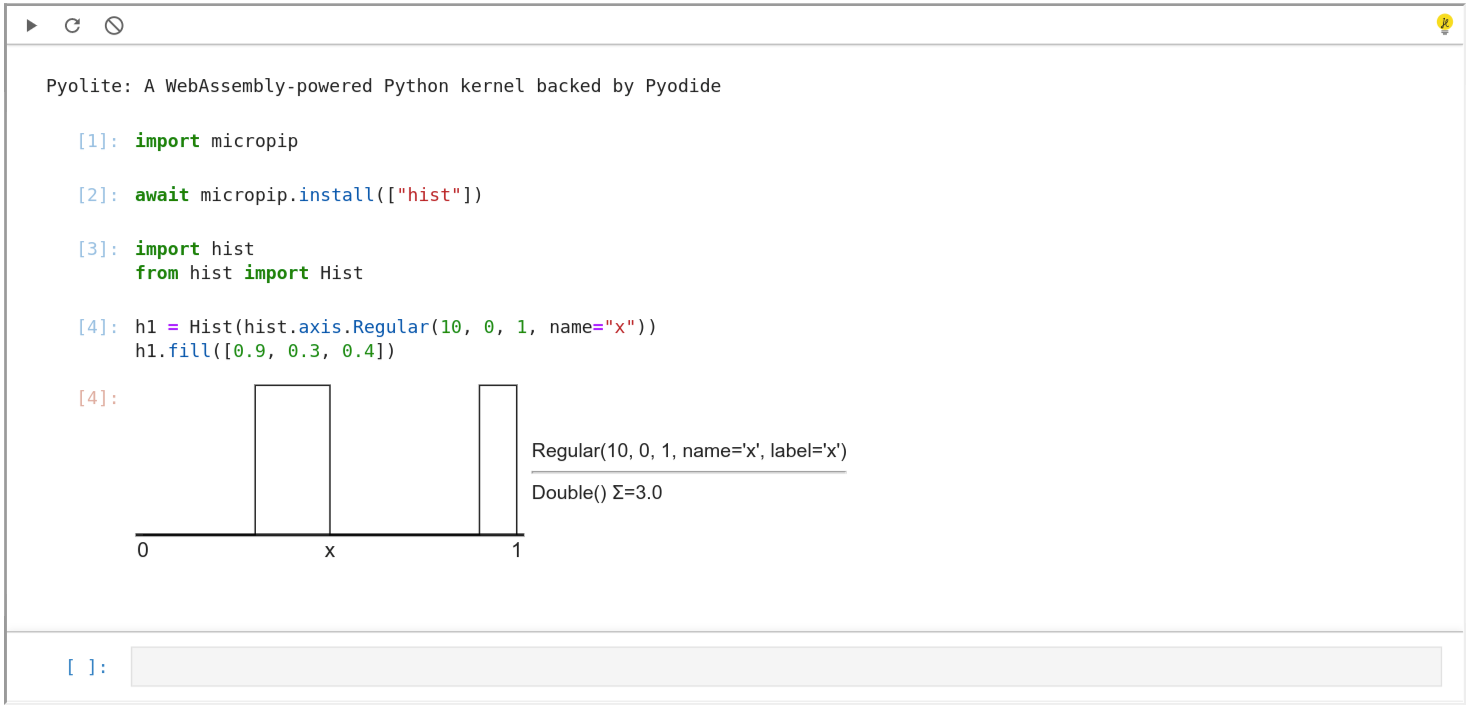
\includegraphics[width=\linewidth]{pyodide-hist.png}}
            {\tiny (\linkref{https://pyodide.org/en/stable/}{Pyodide} CPython port to WebAssembly/Emscripten powering \linkref{https://jupyterlite.readthedocs.io/}{JupyterLite} kernel)}\\boost-histogram and hist were early trials for Pyodide kernel improvements
        \end{center}
    \end{figure}
  \end{columns}

\end{frame}

\begin{frame}
  \frametitle{Analysis Systems Project Highlights: pyhf}

  \begin{itemize}
    \item pyhf
    \item probability model publishing
    \item Highlight wins in HSF with HEPData
  \end{itemize}

\end{frame}

\begin{frame}
  \frametitle{Analysis Systems Project Highlights: cabinetry}

  \begin{itemize}
    \item cabinetry
    \item Analysis Grand Challenge work
  \end{itemize}

\end{frame}

\begin{frame}
  \frametitle{Analysis Systems Project Highlights: Scikit-HEP}

  \begin{itemize}
    \item Continued growth
    \item PyHEP conferences ongoing
    \item Invitations from Scientific Python to get more invovled in borader community
  \end{itemize}

\end{frame}

\begin{frame}
  \frametitle{Analysis Systems Project Fellows}

  \begin{itemize}
    \item Quick highlight of fellow projects
    \item https://iris-hep.org/as.html
    \item Note pyhf-to-combine converter (Steering Board: Danilo Piparo, CMS)
  \end{itemize}

\end{frame}

\begin{frame}
  \frametitle{Analysis Systems: Year 5 Goals}

  \begin{itemize}
    \item Goals for successful Year 5
  \end{itemize}

\end{frame}

\begin{frame}
  \frametitle{Summary}

  \begin{itemize}
    \item Summary
  \end{itemize}

\end{frame}
